 \documentclass[17pt]{article}
\usepackage{fancyhdr} % Required for custom headers
\usepackage{lastpage} % Required to determine the last page for the footer
\usepackage{extramarks} % Required for headers and footers
\usepackage{graphicx} % Required to insert images
\usepackage{lipsum} % Used for inserting dummy 'Lorem ipsum' text into the template
\usepackage{amsmath,amsthm,amsxtra}

% Margins
\topmargin=-0.45in
\evensidemargin=0in
\oddsidemargin=0in
\textwidth=6.5in
\textheight=9.0in
\headsep=0.25in 

\linespread{1.1} % Line spacing

% Set up the header and footer
\pagestyle{fancy}
\lhead{\hmwkAuthorName} % Top left header
\chead{\courseTitle\ : \hmwkTitle} % Top center header
\rhead{\firstxmark} % Top right header
\lfoot{\lastxmark} % Bottom left footer
\cfoot{} % Bottom center footer
\rfoot{Page\ \thepage\ of\ \pageref{LastPage}} % Bottom right footer
\renewcommand\headrulewidth{0.4pt} % Size of the header rule
\renewcommand\footrulewidth{0.4pt} % Size of the footer rule

\setlength\parindent{0pt} % Removes all indentation from paragraphs

%----------------------------------------------------------------------------------------
%	DOCUMENT STRUCTURE COMMANDS
%	Skip this unless you know what you're doing
%----------------------------------------------------------------------------------------

% Header and footer for when a page split occurs within a problem environment
\newcommand{\enterProblemHeader}[1]{
\nobreak\extramarks{#1}{#1 continued on next page\ldots}\nobreak
\nobreak\extramarks{#1 (continued)}{#1 continued on next page\ldots}\nobreak
}

% Header and footer for when a page split occurs between problem environments
\newcommand{\exitProblemHeader}[1]{
\nobreak\extramarks{#1 (continued)}{#1 continued on next page\ldots}\nobreak
\nobreak\extramarks{#1}{}\nobreak
}

\setcounter{secnumdepth}{0} % Removes default section numbers
\newcounter{homeworkProblemCounter} % Creates a counter to keep track of the number of problems
\newcommand{\homeworkProblemName}{}
\newenvironment{homeworkProblem}[1][Problem \arabic{homeworkProblemCounter}]{ % Makes a new environment called homeworkProblem which takes 1 argument (custom name) but the default is "Problem #"
\stepcounter{homeworkProblemCounter} % Increase counter for number of problems
\renewcommand{\homeworkProblemName}{#1} % Assign \homeworkProblemName the name of the problem
\section{\homeworkProblemName} % Make a section in the document with the custom problem count
\enterProblemHeader{\homeworkProblemName} % Header and footer within the environment
}{
\exitProblemHeader{\homeworkProblemName} % Header and footer after the environment
}

\newcommand{\problemAnswer}[1]{ % Defines the problem answer command with the content as the only argument
\noindent\framebox[\columnwidth][c]{\begin{minipage}{0.98\columnwidth}#1\end{minipage}} % Makes the box around the problem answer and puts the content inside
}

\newcommand{\homeworkSectionName}{}
\newenvironment{homeworkSection}[1]{ % New environment for sections within homework problems, takes 1 argument - the name of the section
\renewcommand{\homeworkSectionName}{#1} % Assign \homeworkSectionName to the name of the section from the environment argument
\subsection{\homeworkSectionName} % Make a subsection with the custom name of the subsection
\enterProblemHeader{\homeworkProblemName} % Header and footer within the environment
}{
\enterProblemHeader{\homeworkProblemName} % Header and footer after the environment
}

%----------------------------------------------------------------------------------------
%	NAME AND CLASS SECTION
%----------------------------------------------------------------------------------------

\newcommand{\hmwkTitle}{Assignment 2} % Assignment title
\newcommand{\hmwkDueDate}{Wendesday,\ Feb 18,\ 2013} % Due date
\newcommand{\courseTitle}{Quantum Electronics and Photonics} % Course/class
\newcommand{\hmwkClassInstructor}{Prof. Hamed Majedi} % Teacher/lecturer
\newcommand{\hmwkAuthorName}{Behrooz Semnani} % Your name
\newcommand{\sudentNumber}{20490883} % Your name
\newcommand{\position}{PhD student at ECE departent}

%----------------------------------------------------------------------------------------
%%-----------------------------------------------------------------------------------------

%%%%%%%%%%
\newcommand{\red}[1]{\textcolor[rgb]{1,0,0}{#1}}
\newcommand{\blu}[1]{\textcolor[rgb]{0,0,1}{#1}}
\newcommand{\bs}[1]{\boldsymbol{#1}}
%\newcommand{\V}[1]{\bm{#1}}
\newcommand{\V}[1]{\Vec{#1}}
\newcommand{\A}[1]{\Hat{#1}}
\newcommand{\W}[1]{\widehat{#1}}
\newcommand{\T}[1]{\widetilde{#1}}
\newcommand{\pd}[2]{\dfrac{\partial #1}{\partial #2}}
\newcommand{\fpd}[2]{\frac{\partial #1}{\partial #2}}
\newcommand{\pds}[1]{\dfrac{\partial}{\partial #1}}
\newcommand{\fpds}[1]{\frac{\partial}{\partial #1}}
\newcommand{\pdss}[1]{\dfrac{\partial^2}{\partial {#1}^2}}
\newcommand{\pdsss}[2]{\dfrac{\partial^2}{\partial #1 \partial #2}}
\newcommand{\pdt}[2]{\dfrac{\partial^2 {#1}}{\partial {#2}^2}}
\newcommand{\pdtt}[3]{\dfrac{\partial^2 {#1}}{\partial {#2} \partial {#3}}}
\newcommand{\dif}[2]{\frac{d{#1}}{d{#2}}}
\newcommand{\vt}[1]{\Vec{\mathcal{#1}}}
\newcommand{\VP}[1]{\Vec{\mathbf{#1}}}
\newcommand{\vp}[1]{\mathbf{#1}}
\newcommand{\phas}[1]{\angle{#1}^{\circ}}
\newcommand{\er}{\epsilon_{r}}
\newcommand{\mr}{\mu_{r}}
\newcommand{\Lrw}{\Longrightarrow}
\newcommand{\refeq}[1]{(\ref{#1})}
\newcommand{\abs}[1]{\left| #1\right|}
\newcommand{\ket}[1]{|#1\rangle}
\newcommand{\bra}[1]{\langle #1| }
\newcommand{\bracket}[2]{\langle#1|#2\rangle }
\newcommand{\comut}[2]{\left[#1,#2\right]}

%%%---
\newcommand\ointint{\begingroup
\displaystyle \unitlength 1pt
\int\mkern-7.2mu
\begin{picture}(0,3)
\put(0,3){\oval(10,8)}
\end{picture}
\mkern-7mu\int\endgroup}
%%%----
\providecommand{\abs}[1]{\lvert#1\rvert}
\providecommand{\norm}[1]{\lVert#1\rVert}

%%%%%%%%%%%%%%%

%---Packeges------------------------------------------------------------------
 %------------------------------------------------------
\usepackage[utf8]{inputenc}
\usepackage[T1]{fontenc}
\usepackage[english]{babel}
\usepackage[latin1]{inputenc}
\usepackage[T1]{fontenc}
\usepackage{pstricks}
\usepackage[usenames,dvipsnames]{pstricks}
\usepackage{epsfig}
\usepackage{pst-grad} % For gradients \usepackage{pst-plot} % For axes
\usepackage{pifont}
\usepackage{amsfonts}
\graphicspath{{IMG/}}
\usepackage[utf8]{inputenc}
 \usepackage[OT1]{fontenc}
 \usepackage[absolute,overlay]{textpos}
 \usepackage{graphicx}
 \usepackage[bookmarks=false,pdffitwindow]{hyperref}
 \usepackage{tikz}
 \usepackage{xcolor}
 \usepackage{calc}
\usepackage{chngcntr}
%----------------------------------------------------------------
\numberwithin{equation}{section}
\renewcommand{\theequation}{\arabic{equation}}



%%------------------------------------------------------------------------------------------
%	TITLE PAGE
%----------------------------------------------------------------------------------------

\title{
\vspace{2in}
\textmd{\textbf{\courseTitle\\ \vspace{0.5in}\hmwkTitle}}\\
\vspace{0.5in}\large{{\hmwkClassInstructor}}
\vspace{3in}
}
\author{\textbf{\hmwkAuthorName}\\ 
}\\

\date{February 18, 2013} % Insert date here if you want it to appear below your name

%----------------------------------------------------------------------------------------

\begin{document}

\maketitle


\newpage
\tableofcontents
\newpage


%----Problems-------
\begin{homeworkProblem}

\begin{homeworkSection}{(a)}
To construct the Hamiltonian describing time evolution of the dynamical varibales we can simply consider the total energy of the system as a constant of motion however we firmly follow a more general approach. we first try to redrive the second order differential equation which determines equation of motion based on Lagrange equation. Primary KVL and KCL equations manifest themself in defining conjugate varibales. Quite generally we should first pick up minimum number of varibles which can completely describe the working point in configuration space. We choose $\mathcal{Q}=v$ as the sole dynamical quantity. $i$ is related to $v$ by:
\begin{equation}
i=C\frac{dv}{dt}=C\dot{\mathcal{Q}}
\end{equation}
\begin{figure}[!h]
\centering
% Generated with LaTeXDraw 2.0.8
% Thu Feb 28 09:11:00 GMT-06:00 2013
% \usepackage[usenames,dvipsnames]{pstricks}
% \usepackage{epsfig}
% \usepackage{pst-grad} % For gradients
% \usepackage{pst-plot} % For axes
\scalebox{0.7} % Change this value to rescale the drawing.
{
\begin{pspicture}(0,-1.5479687)(4.9146876,1.5879687)
\psline[linewidth=0.028222222cm](3.8764584,0.9753869)(3.8864996,0.56300914)
\rput{-88.605156}(3.507715,4.24715){\psarc[linewidth=0.028222222](3.9297698,0.32649234){0.2}{0.0}{180.0}}
\rput{-88.605156}(3.916978,3.8667367){\psarc[linewidth=0.028222222](3.9395065,-0.07338913){0.2}{0.0}{180.0}}
\rput{-88.605156}(4.3262405,3.486323){\psarc[linewidth=0.028222222](3.9492435,-0.4732706){0.2}{0.0}{180.0}}
\rput{-88.605156}(4.7366757,3.073829){\psarc[linewidth=0.028222222](3.9431307,-0.8897928){0.18375}{0.0}{180.0}}
\psline[linewidth=0.028222222cm](3.9272726,-1.1114945)(3.9373138,-1.5238723)
\psline[linewidth=0.04cm](3.936875,-1.5279688)(1.356875,-1.5279688)
\psline[linewidth=0.04cm](3.876875,0.97203124)(1.296875,0.97203124)
\psline[linewidth=0.054cm](1.756875,-0.098767914)(0.916875,-0.098767914)
\psline[linewidth=0.054cm](1.756875,-0.38796875)(0.916875,-0.38796875)
\psline[linewidth=0.04cm](1.316875,0.95203125)(1.336875,-0.04796875)
\psline[linewidth=0.04cm](1.376875,-1.5279688)(1.376875,-0.38796875)
\psline[linewidth=0.04cm,arrowsize=0.133cm 2.36,arrowlength=1.4,arrowinset=0.4]{<-}(2.236875,0.9521436)(2.576875,0.9519189)
\usefont{T1}{ptm}{m}{n}
\rput(2.1842186,-0.27296874){\large $C$}
\usefont{T1}{ptm}{m}{n}
\rput(4.534219,-0.29296875){\large $L$}
\usefont{T1}{ptm}{m}{n}
\rput(2.5142188,1.3670312){\large $i$}
\usefont{T1}{ptm}{m}{n}
\rput(0.28421876,-0.25296876){\large $v$}
\end{pspicture} 
}

\caption{\small parallel LC network}
\end{figure}
Please note that we could also choose the cahrge of the capacitor ($Q$) and total magnetic flux inisde the inductor ($\Phi$) as the dynamical variables. We define the action as the difference of magnetic and electrical energies as:
\begin{equation}
\mathcal{L}=\frac{1}{2}Li^2-\frac{1}{2}Cv^2=\frac{1}{2}C\left[\frac{1}{\omega_0^2}\dot{\mathcal{Q}}^2-\mathcal{Q}^2\right]
\end{equation}  
where $\omega_0$ is defined as 
$$\omega_0=\frac{1}{\sqrt{LC}}$$
Lagrange equation for this action is:
\begin{equation}
\frac{d}{dt}\pd{\M{L}(\M{Q},\dot{\M{Q}})}{\dot{\M{Q}}}-\pd{\M{L}(\M{Q},\dot{\M{Q}})}{\M{Q}}=0\quad\Lrw\quad \ddot{\M{Q}}=-\omega_0^2\M{Q}\quad\Lrw\quad \frac{d^2v}{dt^2}=-\omega_0^2 v
\end{equation}
This equation is exactly same as the equation which can be derived based on KVL and KCL equations. Thus our Lagrangian works well and we can go ahead to cunstruct the Hamiltonian. First note that the conjugate varible corresponde to  $\M{Q}$ is:
\begin{equation}
\M{P}=\pd{\M{L}}{\dot{\M{Q}}}=\frac{C\dot{\M{Q}}}{\omega_0^2}=LC i
\end{equation}
Now the Hamiltonian is:
\begin{equation}\label{P1-H}
\M{H}=\left.\M{P}\dot{\M{Q}}-\M{L}(\M{Q},\dot{\M{Q}})\right|_{\dot{\M{Q}}=\omega_0^2\M{P}/C}
=\frac{\omega_0^2\M{P}^2}{2C}+\frac{1}{2}C\M{Q}^2
\end{equation}
Interestingly canonical equations of motion in phase space are:
\begin{align}
\dot{\M{Q}}=\pd{\M{H}(\M{Q},\M{P})}{\M{P}}=\frac{\omega_0^2\M{P}}{C}\quad  &\Lrw \quad   C\frac{dv}{dt}=i \quad\text{(KCL)}\\
\dot{\M{P}}=-\pd{\M{H}(\M{Q},\M{P})}{\M{Q}}=-C\M{Q}\quad &\Lrw \quad  L\frac{di}{dt}=-v \quad \text{(KVL)}
\end{align}
\end{homeworkSection}
\begin{homeworkSection}{(b)}
The Hamiltonian describing time evolution in a one dimensional SHO is:
\begin{equation}\label{P1-SHO}
H=\frac{p^2}{2m}+\frac{1}{2}m\omega^2x^2
\end{equation}
where $x$ and $p$ are conjugate varibles. In both \eqref{P1-H} and \eqref{P1-SHO} Hamiltonians are elipitical functions of two conjugate varibles. In fact both Hamiltonians are equal if we do the following replacements:
\begin{equation}\label{P1-Sub}
H\leftrightarrow \M{H}\qquad x\leftrightarrow\M{Q}\qquad p\leftrightarrow\M{P}\qquad m\leftrightarrow LC^2\qquad\omega\leftrightarrow \omega_0
\end{equation}

 \end{homeworkSection}

\begin{homeworkSection}{(c)}
 The conh=jugate varible to $\M{Q}=v$ has been calculated in part (a) as we showed:
 \begin{equation}
 \M{P}=\pd{\M{L}}{\dot{\M{Q}}}=\frac{C\dot{\M{Q}}}{\omega_0^2}=LC i
 \end{equation}
 \end{homeworkSection}

%--------d--------------
\begin{homeworkSection}{(d)}
To quantize the LC circuit we start form the Driac's quantization rules. We first take a look at fundamental Poison backets in the classical problem:
\begin{equation}
\left\{\M{Q},\M{P}\right\}=\pd{\M{Q}}{\M{Q}}\pd{\M{P}}{\M{P}}-\pd{\M{P}}{\M{Q}}\pd{\M{Q}}{\M{P}}=1
\end{equation}   
According to the Dirac's quantization rule we should just replace:
\begin{equation}
\frac{1}{j\hbar}\left[\quad ,\quad \right]\leftrightarrow\left\{\quad,\quad\right\}
\end{equation}
Please note that we have used $j$ as the unit imaginary number. This quantization implies that $\M{Q}$ and $\M{P}$ should be treated as operators. So we have:
\begin{equation}
\left[\A{\M{Q}},\A{\M{P}}\right]=\left[\A{v},LC\A{i}\right]=j\hbar
\end{equation}
This commutation relation is the starting point to develop the whole \textit{Lie algebra}. So we should have the same quantization and generally algebra in a SHO and quantum LC circuit.
\end{homeworkSection}



%------------e-------------
\begin{homeworkSection}{(e)} 
As it's explained in the previous part we have the same algebra in SHO and quantum LC network. So we can simply use the result of our discussions in SHO. we should just use the substitutions given in \eqref{P1-Sub}. So we have:
\begin{align}
&a_{SHO}=\sqrt{\frac{m\omega}{2\hbar}}\left(x+\frac{jp}{m\omega}\right)\quad\Lrw\quad 
\M{A}=\sqrt{\frac{LC^2\omega_0}{2\hbar}}\left(\M{Q}+\frac{j\M{P}}{LC^2\omega_0}\right)\\
&a^\dagger_{SHO}=\sqrt{\frac{m\omega}{2\hbar}}\left(x-\frac{jp}{m\omega}\right)\quad\Lrw\quad 
\M{A}^{\dagger}=\sqrt{\frac{LC^2\omega_0}{2\hbar}}\left(\M{Q}-\frac{j\M{P}}{LC^2\omega_0}\right)
\end{align}
 or
 \begin{align}
 \M{A}&=\sqrt{\frac{C}{2\hbar\omega_0}}\left(\A{v}+\frac{j\A{i}}{C\omega_0}\right)\qquad \text{annihilation operator}\label{P1-111}\\
 \M{A}^{\dagger}&=\sqrt{\frac{C}{2\hbar\omega_0}}\left(\A{v}-\frac{j\A{i}}{C\omega_0}\right)\qquad\text{creation operator}\label{P1-112}
 \end{align}
The Hamiltonian can be rewriten in terms of creation and annihilation operators as:
\begin{equation}
\M{H}=\hbar \omega_0\left(\M{A}^{\dagger}\M{A}+\frac{1}{2}\right)
\end{equation}
Numbering operator is defined as:
\begin{equation}
\M{N}=\M{A}^{\dagger}\M{A}
\end{equation}

\end{homeworkSection}
%-----f-----------
\begin{homeworkSection}{(f)}
from \eqref{P1-111} and \eqref{P1-112}
\begin{align}
\A{v}&=\sqrt{\frac{\hbar\omega_0}{2C}}\left(\M{A}+\M{A}^{\dagger}\right)\\
\A{i}&=-j\sqrt{\frac{\hbar\omega_0}{2L}}\left(\M{A}-\M{A}^{\dagger}\right)
\end{align}

\end{homeworkSection}
%-----g-----
\begin{homeworkSection}{(g)}
Using the results of the quantization of SHO we can write:
\begin{equation}
E_n=\left(n+\frac{1}{2}\right)\hbar\omega_0=\left(n+\frac{1}{2}\right)\hbar\frac{1}{\sqrt{LC}}
\end{equation}
\end{homeworkSection}

%------h------
\begin{homeworkSection}{(h)}
Current and voltage as conjugate dynamical varibles are incompatible. So the following uncertainty relations prohibite the precise measurment of both $v$ and $i$ simultaniously:
\begin{equation}
\langle(\Delta v)^2\rangle\langle (\Delta i)^2\rangle\geq\frac{1}{4}\left|\langle\left[\A{v},\A{i}\right]\rangle\right|^2=\frac{\hbar^2}{4L^2C^2}
\end{equation}
Paricularly uncertainty in nth energy eigenstate is:
\begin{align}
&\langle(\Delta v)^2\rangle_n=\bra{n} v^2\ket{n} -\bra{n} v\ket{n}^2=\frac{\hbar\omega_0}{2C}\bra{n}\M{A}^2+\M{A}^{\dagger}^2+\M{A}\M{A}^{\dagger}+\M{A}^{\dagger}\M{A}\ket{n}-\frac{\hbar\omega_0}{2C}\bra{n}\M{A}+\M{A}^{\dagger}\ket{n}^2\\
&\langle(\Delta i)^2\rangle_n=\bra{n} i^2\ket{n} -\bra{n} i\ket{n}^2=\frac{\hbar\omega_0}{2L}\bra{n}\M{A}^2+\M{A}^{\dagger}^2+\M{A}\M{A}^{\dagger}+\M{A}^{\dagger}\M{A}\ket{n}-\frac{\hbar\omega_0}{2L}\bra{n}\M{A}+\M{A}^{\dagger}\ket{n}^2
\end{align}
Hence:
\begin{equation}\label{P1-220}
\left.
\begin{array}{l}
\langle(\Delta v)^2\rangle_n =\frac{\hbar\omega_0}{2C}(2n+1)\\
\langle(\Delta i)^2\rangle_n =\frac{\hbar\omega_0}{2L}(2n+1)
\end{array}
\right\}\quad\Lrw\quad \langle(\Delta v)^2\rangle_n\langle(\Delta i)^2\rangle_n=\frac{\hbar^2}{4L^2C^2}(2n+1)^2
\end{equation}
Clearly qunatum uncertainty which reprsents quantum mechanical effects is proportional to $\omega_0^4$ this menas that quantum mechanical effects are more important at higher frequencies comparable to $\omega_0$. Dimensional analysis is a direct method to show this limit.  
\end{homeworkSection}

\begin{homeworkSection}{(i)}
To evaluate quantum flactuation level in an eigenstate of energy we use equation \eqref{P1-220}. We have:
\begin{align}
&\sqrt{\langle(\Delta v)^2\rangle_n}=\sqrt{\frac{\hbar\omega_0}{2C}(2n+1)}\approx 1.28 \mathrm{\mu V}\sqrt{2n+1}\\
&\sqrt{\langle(\Delta i)^2\rangle_n}=\sqrt{\frac{\hbar\omega_0}{2L}(2n+1)}\approx 40.7 \mathrm{nA}\sqrt{2n+1}
\end{align}
\end{homeworkSection}
%-----j----------------------------
\begin{homeworkSection}{(j)}
We assume that quanta of thermal radiation is $k_BT$. $k_B$ is Boltzman's constant. To measure the the quantized energy levels we should conduct our experiment in an enviornment in which termal energy quanta is lower than the half of the first energy level:
\begin{equation}
k_BT<\frac{\hbar\omega_0}{2}\quad\Lrw\quad T<0.12\mathrm{K}
\end{equation} 
%--------
\end{homeworkSection}
%----k----
\begin{homeworkSection}{(k)}
Assume that the voltage wave function is reptresented by $\Psi(v,t)$. since $\M{Q}$ and $\M{P}$ commutation relation is the same as $x-p$ commutation relation we can use the same math. So we can just replace $\M{P}\leftrightarrow -j\hbar\fpds{\M{Q}}$. Hamiltonian is also generator of time translation so we can write:
\begin{equation}
j\hbar\pd{\Psi(v,t)}{t}=-\frac{\omega_0^2\hbar^2}{2C}\pdt{\Psi(v,t)}{v}+\frac{1}{2}Cv^2\Psi(v,t)
\end{equation}
\end{homeworkSection}
%-----l------
\begin{homeworkSection}{(l)}
The voltage wavefunction associated with the ground state of the LC network is similar to x-space wave function of SHO. we should just use \eqref{P1-Sub}. Actually we have:
\begin{equation}
\M{A}\ket{0}=0\quad\Lrw\quad v\Psi_0(v)+\frac{\hbar}{LC^2\omega_0}\pd{\Psi_{0}(v)}{v}=0
\end{equation}
And explicitly:
\begin{equation}
\Psi_0(v)=\left({\frac{LC^2\omega_0}{\pi\hbar}}\right)^{1/4}\exp\left[-\frac{1}{2}\frac{LC^2\omega_0 v^2}{\hbar}\right]
\end{equation}

\end{homworkSection}


\end{homeworkProblem}

\setcounter{equation}{0}
%----------------
\begin{homeworkProblem}
\begin{homeworkSection}{(a)}
Strating with
\begin{equation*}
[\A{a},\A{a}^\dagger]=1
\end{equation*}
we arrive at:
\begin{equation}\label{P2-1}
[\A{N},\A{a}^\dagger]=[\A{a}^\dagger\A{a},\A{a}^\dagger]=\A{a}^\dagger[\A{a},\A{a}^\dagger]+[\A{a}^\dagger,\A{a}^\dagger]\A{a}=\A{a}^\dagger
\end{equation}
Note that in \eqref{P2-1} we have used the following identity:
\begin{equation}\label{P2-i}
[\A{A}\A{B},\A{C}]=\A{A}[\A{B},\A{C}]+[\A{A},\A{C}]\A{B}
\end{equation}
In the same line of reasoning we get:
\begin{equation}
[\A{N},\A{a}]=[\A{a}^\dagger\A{a},\A{a}]=\A{a}^\dagger[\A{a},\A{a}]+[\A{a}^\dagger,\A{a}]\A{a}=-\A{a}
\end{equation}
\end{homeworkSection}
\begin{homeworkSection}{(b)}
In the prsence of nonlinearity the Hamiltonian is:
\begin{equation}
\A{H}=\hbar\omega_0\A{a}^\dagger\A{a}-\frac{\hbar\kappa}{2}\A{a}^\dagger\A{a}^\dagger\A{a}\A{a}
\end{equation}
hence:
\begin{equation}
[\A{N},\A{H}]=[\A{a}^\dagger\A{a},\hbar\omega_0\A{a}^\dagger\A{a}-\frac{\hbar\kappa}{2}\A{a}^\dagger\A{a}^\dagger\A{a}\A{a}]=
-\frac{\hbar\kappa}{2}[\A{N},\A{a}^\dagger\A{a}^\dagger\A{a}\A{a}]
\end{equation}
Successive application of \eqref{P2-i} we can write:
\begin{align}
[\A{N},\A{a}^\dagger\A{a}^\dagger\A{a}\A{a}] &=\A{a}^\dagger [\A{N},\A{a}^\dagger\A{a}\A{a}]+[\A{N},\A{a}^\dagger]\A{a}^\dagger\A{a}\A{a}\\
[\A{N},\A{a}^\dagger\A{a}\A{a}]  &=  \A{a}^\dagger[\A{N},\A{a}\A{a}]+[\A{N},\A{a}^\dagger]\A{a}\A{a}\\
[\A{N},\A{a}\A{a}] &=\A{a}[\A{N},\A{a}]+[\A{N},\A{a}]\A{a}
\end{align} 
So we have:
\begin{equation}
[\A{N},\A{a}^\dagger\A{a}^\dagger\A{a}\A{a}]=-2\A{a}^\dagger\A{a}^\dagger\A{a}\A{a}+2\A{a}^\dagger\A{a}^\dagger\A{a}\A{a}=0
\end{equation}
combining all we get:
\begin{equation}\label{P2-NH}
[\A{N},\A{H}]=0
\end{equation}
We can employ a simpler analysis as well. If we write the Hamiltonian in the following form:
\begin{equation*}
\A{H}=\hbar\omega_0\A{N}-\frac{\hbar\kappa}{2}\A{a}^\dagger\A{N}\A{a}
\end{equation*}
using \eqref{P2-1} we can write:
\begin{equation}\label{P2-500}
\A{H}=\hbar\omega_0\A{N}-\frac{\hbar\kappa}{2}\left(\A{N}\A{a}^\dagger-\A{a}^\dagger\right)\A{a}=
\hbar\omega_0\A{N}-\frac{\hbar\kappa}{2}\left(\A{N}^2-\A{N}\right)
\end{equation}
We can readily see that the Hamiltonian is a function number operator and equation \eqref{P2-NH} holds. 
\end{homeworkSection}
%----------------------c---------
\begin{homeworkSection}{(c)}
Since $\A{N}$ and $\A{H}$ commutate , they can be simultaneously diagonalize. Eigenstates of the number operator are not degenerate so we can use number operator basis function as the eigenstates of the Hamiltonian:
\begin{equation}
\A{H}\ket{n}=\hbar\omega_0 n\ket{n}-\frac{\hbar\kappa}{2}\A{a}^\dagger\A{a}^\dagger\A{a}\A{a}\ket{n}
\end{equation} 
Using
\begin{equation*}
\A{a}\ket{n}=\sqrt{n}\ket{n-1}\qquad\A{a}^\dagger\ket{n}=\sqrt{n+1}\ket{n+1}
\end{equation*}
we obtain:
\begin{equation}
\A{a}^\dagger\A{a}^\dagger\A{a}\A{a}\ket{n}=\sqrt{n(n-1)(n-1)n}\ket{n}=n(n-1)\ket{n}
\end{equation}
So we have:
\begin{equation}
\A{H}\ket{n}=\left\{\hbar\omega_0 n-\frac{\hbar\kappa}{2}n(n-1)\right\}\ket{n}
\end{equation}
we could also use \eqref{P2-500} which leads to the same result:
\begin{equation}\label{P2-550}
\A{H}\ket{n}=\hbar\omega_0\A{N}\ket{n}-\frac{\hbar\kappa}{2}\left(\A{N}^2-\A{N}\right)\ket{n}=
\left\{\hbar\omega_0 n-\frac{\hbar\kappa}{2}n(n-1)\right\}\ket{n}
\end{equation}
\end{homeworkSection}
%----------d-----------
\begin{homeworkSection}{(d)}
We have already proved that $\A{N}$ and $\A{H}$ commute. So we can immediately conclude that the number operator is a constant of motion. The Hesenberg time evolution for number operator is:
\begin{equation}
\frac{d\A{N}}{dt}=\frac{1}{i\hbar}[\A{N},\A{H}]=0\quad\Lrw\quad \A{N}=\A{N}(0)
\end{equation}
Since $\A{N}$ is a constant motion the number photons inside the cavity remains constant during time evolution.
\end{homeworkSection}
\begin{homeworkSection}{(e)}
The Heisenberg time evolution equation for the annihilation operator is:
\begin{equation}
\frac{d\A{a}}{dt}=\frac{1}{i\hbar}[\A{a},\A{H}]=-i[\A{a},\omega\A{N}-\frac{\kappa}{2}\A{a}^\dagger\A{a}^\dagger\A{a}\A{a}]=-i\omega_0\A{a}+\frac{i\kappa}{2}[\A{a},\A{a}^\dagger\A{a}^\dagger\A{a}\A{a}]
\end{equation}
Using \eqref{P2-i} identity we obtain:
\begin{equation}
[\A{a},\A{a}^\dagger\A{a}^\dagger\A{a}\A{a}]=\A{a}^\dagger\A{a}^\dagger[\A{a},\A{a}\A{a}]+[\A{a},\A{a}^\dagger\A{a}^\dagger]\A{a}\A{a}=2\A{a}^\dagger\A{a}\A{a}=2\A{N}\A{a}
\end{equation}
Since $\A{N}$ is a constant of motion we can write:
\begin{equation}\label{P2-a}
\frac{d\A{a}(t)}{dt}=-i\omega_0\A{a}(t)+i\kappa\A{N}(0)\A{a}(t)
\end{equation} 
To solve this first order differential equation we define am auxiliary operator:
\begin{equation}
\A{\zeta}(t)=\A{a}(t)\exp(i\omega_0 t)
\end{equation}
Inserting in \eqref{P2-a} we obtain:
\begin{equation}
\frac{d\A{\zeta}(t)}{dt}=i\kappa \A{N}(0)\A{\zeta}(t)
\end{equation}
So we arrive at:
\begin{equation}
\A{\zeta}(t)=e^{i\kappa\A{N}(0)t}\A{\zeta(0)}
\end{equation}
finally we get:
\begin{equation}\label{P2-at}
\A{a}(t)=\exp\left[-i\omega_0t+i\kappa\A{N}(0)t\right]\A{a}(0)
\end{equation}
\end{homeworkSection}
%-----------------f----------------------------
\begin{homeworkSection}{(f)}
Applying transpose conjugate operator on both sides of \eqref{P2-at} we obtain:
\begin{equation}
\A{a}^\dagger(t)=\A{a}^\dagger(0)\exp\left[i\omega_0t-i\kappa\A{N}^\dagger(0)t\right]=\A{a}^\dagger(0)\exp\left[i\omega_0t-i\kappa\A{N}(0)t\right]
\end{equation}
From operator algebra we know that :
\begin{equation}
[A,B]=\lambda A\quad\Lrw\quad Ae^{B}=e^\lambda e^B A
\end{equation}
Since $[\A{a}^\dagger(0),\A{N}(0)]=-\A{a}^\dagger(0)$ then:
\begin{equation}
\A{a}^\dagger(t)=\exp\left[i\kappa t+i\omega_0t-i\kappa\A{N}(0)t\right]\A{a}^\dagger(0)
\end{equation}
\end{homeworkSection}
%----------------------g------------
\begin{homeworkSection}{(g)}
If just one photon is lost from the cavity total energy of the system inside the cacity would change. We can simply calculate the energy difference  in the number state. Before $t=T$ the quantum state of the field is given by $\ket{n}$ and  by photon annihilation the state in the nuumber state would be $\ket{n-1}$ so we have:  
\begin{equation}
\hbar\omega_{ph}=\Delta E=E_1-E_2=\bra{n}\A{H}\ket{n}-\bra{n-1}\A{H}\ket{n-1}
\end{equation}
Using \eqref{P2-550} we can write:
\begin{eqnarray}
\Delta E&=&\left\{\hbar\omega_0 n-\frac{\hbar\kappa}{2}n(n-1)\right\}-\left\{\hbar\omega_0 (n-1)-\frac{\hbar\kappa}{2}(n-1)(n-2)\right\}\nonumber\\
&=&\hbar\omega_0-\hbar\kappa(n-1)
\end{eqnarray}
So the spectrometer measures:
\begin{equation}
\omega_{ph}=\frac{\Delta E}{\hbar}=\omega_0-\kappa(n-1)
\end{equation}
Note that we can measure the frequency with certainty.
\end{homeworkSection}


\end{homeworkProblem}
\setcounter{equation}{0}
%---------------
\newpage
\begin{homeworkProblem}
The spinor part of the Hamiltonian describing time evolution of  an half spin system such as electron inside a uniform but time-varying magnetic filed is:
\begin{equation}
H=-\B{\mu}.\vp{B}=-\frac{gq}{2m}\vp{S}.\vp{B}=-\mu_0\B{\sigma}.\vp{B}
\end{equation}
 where $g$ is gyromagnetic ration and $\mu_0$ is defined as:
 \begin{equation}
 \mu_0=\frac{qg}{2m}
 \end{equation}
Explicitly the Hamiltonian is:
\begin{equation}
H=-\mu_0B_0
\begin{pmatrix}
\cos\theta & \sin\theta\left[\cos\omega t-i\sin\omega t\right]\\
\sin\theta\left[\cos\omega t+i\sin\omega t\right] & -\cos\theta
\end{pmatrix}
\end{equation} 
For notational convenience we write the Hamiltonian in terms of two new parameters:
\begin{equation}
H=-\hbar
\begin{pmatrix}
\omega_1              & \gamma e^{-i\omega t}\\
\gamma e^{i\omega t} & -\omega_1 
\end{pmatrix}
\end{equation}
where:
\begin{align*}
\hbar\omega_1 &=\mu_0B_0\cos\theta\\
 \hbar\gamma &=\mu_0B_0\sin\theta
\end{align*}
The Schr\"odinger equation now reads:
\begin{equation}\label{P3-S}
i\hbar\frac{d}{dt}
\begin{pmatrix}
c_1(t)\\
c_2(t)
\end{pmatrix}
=
-\hbar\begin{pmatrix}
\omega_1              & \gamma e^{-i\omega t}\\
\gamma e^{i\omega t} & -\omega_1 
\end{pmatrix}
\begin{pmatrix}
c_1(t)\\
c_2(t)
\end{pmatrix}
\end{equation}
In the absense of the time dependent part of the Hamiltonian the solution is simply $c_1(t)=A\exp(i\omega_1 t)$ and $c_2(t)=B\exp(-i\omega_1 t)$. It's reasonable to keep the exponential part for the new Hamiltonian. Two coupled first order differential equations given in \eqref{P3-S} can be extremely simplified by the following change of varibles:
\begin{equation}
c_1(t)=A(t)\exp(i\omega_1 t)\qquad  c_2(t)=B(t)\exp(-i\omega_1 t)
\end{equation}   
Two new coupled equations are:  
\begin{equation}
\left\{
\begin{array}{l}
i\frac{dA(t)}{dt}=-\gamma \exp\left[-i(\omega +2\omega_1)t\right]B(t)\\
i\frac{dB(t)}{dt}=-\gamma \exp\left[+i(\omega +2\omega_1)t\right] A(t)
\end{array}\right.
\end{equation}
If we solve $B(t)$ from the first equation and put it in the second one, we obtain:
\begin{equation}
\frac{d^2A}{dt^2}+i\alpha \frac{dA}{dt}+\gamma^2 A=0
\end{equation}
where $\alpha$ has been defined for notational convenience:
\begin{equation}
\alpha=\omega+2\omega_1
\end{equation}
because of symmetry the same equation holds for $B(t)$ we should change the sign of $\alpha$:
\begin{equation}
\frac{d^2B}{dt^2}-i\alpha \frac{dB}{dt}+\gamma^2 B=0
\end{equation}  
The general solution for two differential equations are simply:
\begin{align}
&A(t)=A_{+} \exp(i\Omega_+t)+A_-\exp(i\Omega_-t)\\
&B(t)=B_+\exp(-i\Omega_+t)+B_-\exp(-i\Omega_-t)
\end{align}
where $\Omega_+$ and $\Omega_-$ are defined as:
\begin{equation}
\Omega_\pm=-\frac{\alpha}{2}\pm\sqrt{\frac{\alpha^2}{4}+\gamma^2}
\end{equation}
The constant coefficients can be writen in terms of $A(0)$ and $B(0)$ :
\begin{equation}
\left\{
\begin{array}{rcl}
A(0) &=&A_++A_- &\\
B(0) &=&B_++B_- &\\
\left.\frac{dA}{dt}\right|_{t=0}=i\gamma B(0)&=&+i\Omega_+A_++i\Omega_-A_-\\
\left.\frac{dB}{dt}\right|_{t=0}=i\gamma A(0)&=&-i\Omega_+B_+-i\Omega_-B_-
\end{array}\right.
\end{equation}
These eqquation lead to:
\begin{align}
A_+&=\frac{\Omega_+ A(0)-\gamma B(0)}{\Omega_+-\Omega_-}\\
A_-&=-\frac{\Omega_+ A(0)-\gamma B(0)}{\Omega_+-\Omega_-}\\
B_+&=-\frac{\Omega_- B(0)+\gamma A(0)}{\Omega_+-\Omega_-}\\
B_-&=\frac{\Omega_+ B(0)+\gamma a(0)}{\Omega_+-\Omega_-}
\end{align}
This problem is a general spin procession problem which shows that a time varying magnetic filed which rotates along a prescribed axis changes the spin state by two diferent frequency components. 
\end{homeworkProblem}
\setcounter{equation}{0}
%-----------------
\begin{homeworkProblem}
\begin{homeworkSection}{(a)}
The Schr\"odinger equation in the presence of electromagnetic field is:
\begin{equation}\label{P4-1}
\frac{1}{2m}\left[-i\hbar\nabla-q\vp{A}\right].\left[-i\hbar\nabla-q\vp{A}\right]\Psi(\vp{r},t)+q\Phi\Psi(\vp{r},t)=i\hbar\pd{\Psi(\vp{r},t)}{t}
\end{equation} 
%---------------
The electrical current desnsity function should describe the follow of the electrical charge so it should be consistent with clssical counterpart. It's reasonable to assume that density of electrical chrage should be $\rho=q\abs{\Psi}^2$ . Moreover current and charge density should satisfy continuity equation:
\begin{equation}
\nabla.\vp{J}=-\pd{\rho}{t}=-q\pd{\abs{\Psi(\vp{r},t)}}{t}
\end{equation}
Mutiplying \eqref{P4-1} by $\Psi^*(\vp{r},t)$ leads to:
\begin{equation}
\Re\left\{\Psi^*\pd{\Psi}{t}\right\}=\frac{1}{2m}\Re\left\{i\hbar\Psi^*\nabla^2\Psi-\frac{i}{\hbar}q^2 \vp{A}^2\abs{\Psi}^2+ q\Psi^*\nabla.(\vp{A}\Psi)+q\Psi^*\vp{A}.\nabla\Psi\right\}
\end{equation}
Making use of divercence identity we have:
\begin{equation}
\nabla.\left(\vp{A}\abs{\Psi}^2\right)=\Psi^*\nabla.(\vp{A}\Psi)+\Psi^*\vp{A}.\nabla\Psi+\Psi\nabla.(\vp{A}\Psi^*)+\Psi^*\vp{A}.\nabla\Psi^*
\end{equation}
therefore:
\begin{equation}
\pd{\abs{\Psi}^2}{t}=\Psi^*\pd{\Psi}{t}+\Psi\pd{\Psi^*}{t}=\frac{\hbar}{2mi}\nabla.\left(\Psi^*\nabla\Psi-\Psi\nabla\Psi^*\right)-\frac{q}{m}\nabla.\left(\vp{A}\abs{\Psi}^2\right)
\end{equation}
So from the continuty equation the best choice for $\vp{J}$ is:
\begin{equation}\label{P4-20}
\vp{J}=\frac{q\hbar}{m}\Im\left\{\Psi^*\nabla\Psi\right\}-\frac{q^2}{m}\vp{A}\abs{\Psi}^2
\end{equation}
If the wave function of the system  is given by:
\begin{equation}
\Psi(r,t)=\sqrt{n(\vp{r},t)}\exp\left[i\theta(\vp{r},t)\right]
\end{equation}
So the gradient of $\Psi$ is:
\begin{equation}\label{P4-110}
\nabla\Psi(\vp{r},t)=\frac{\nabla n(\vp{r},t)}{2\sqrt{n(\vp{r},t)}}\exp\left[i\theta(\vp{r},t)\right]+i\nabla\theta(\vp{r},t)\Psi(\vp{r},t)
\end{equation}
Inserting \eqref{P4-110} into \eqref{P4-20} leads to the following equality:
\begin{equation}
\vp{J}=\frac{q\hbar}{m}\Im\left\{\frac{\nabla n(\vp{r},t)}{2\sqrt{n(\vp{r},t)}}+in(\vp{r},t)\nabla\theta(\vp{r},t)\right\}-\frac{q^2}{m}n(\vp{r},t)\vp{A}
\end{equation}
So we arrive at:
\begin{equation}\label{P4-300}
\vp{J}=qn(\vp{r},t)\left[\frac{\hbar}{m}\nabla\theta(\vp{r},t)-\frac{q}{m}\vp{A}(\vp{r},t)\right]
\end{equation}
\end{homeworkSection}
%----------------b----------------------
\begin{homeworkSection}{(b)}
In fact  we derived  \eqref{P4-300} based on continuty equation , however we can check it here.  If the divergence operator actos on $\vp{J}$ then:
\begin{equation}\label{P4-J}
\nabla.\vp{J}=q\nabla n(\vp{r},t).\left[\frac{\hbar}{m}\nabla\theta(\vp{r},t)-\frac{q}{m}\vp{A}(\vp{r},t)\right]+
q n(\vp{r},t)\left[\frac{\hbar}{m}\nabla^2\theta(\vp{r},t)-\frac{q}{m}\nabla.\vp{A}(\vp{r},t)\right]
\end{equation}  
and equivalent chrage density is:
\begin{equation}\label{P4-505}
\Im\left\{i\hbar\Psi^*\pd{\Psi}{t}\right\}=
\frac{1}{2m}\Im\left\{-\hbar^2\Psi^*\nabla^2\Psi+q^2 \vp{A}^2\abs{\Psi}^2+i\hbar q\abs{\Psi}^2\nabla.\vp{A}+2i\hbar q\Psi^*\vp{A}.\nabla\Psi\right\}
\end{equation}
$\nabla^2 \Psi$ in terms of $n$ and $\theta$ is:
\begin{equation}
\nabla^2\Psi=e^{i\theta}\left[\nabla^2 \sqrt{n}+\frac{i}{\sqrt{n}}\nabla n.\nabla\theta+i\sqrt{n}\nabla^2\theta-\sqrt{n}(\nabla\theta)^2\right]
\end{equation}
So the left hand side of \eqref{P4-505} can be simplified as:
\begin{equation}\label{P4-r}
\text{LHS}=\frac{\hbar}{2m}\left\{-\hbar(\nabla n.\nabla\theta)+\hbar\nabla^2\theta+q n\nabla.\vp{A}+ q \vp{A}.\nabla n\right\}
\end{equation}
From \eqref{P4-J} and \eqref{P4-r} we conclude:
\begin{equation}
\nabla.\vp{J}=-2q\Re\left\{\Psi^*\pd{\Psi}{t}\right\}=-\pd{\rho}{t}
\end{equation}
\end{homeworkSection}
%-----------------c--------------------------
\begin{homeworkSection}{(c)}
The continuity equation implies that $\abs{\Psi}^2$ reprsents the spatial distribution of the charge. In fact amplitude of the wave function in bohm interpretation of qunatum mechanics represents the relative probabilty to find the particle in spacific location. So this quantity can be consider as a measure of the cloud of the charge distribution.    
\end{homeworkSection}
%-----------------e-------------
\begin{homeworkSection}{(e)}
In a smaple of superconductor the wave function is 
\begin{equation}
\Psi(\vp{r},t)=\sqrt{n^*} e^{i\theta(\vp{r},t)}
\end{equation}
where $n^*$ is constant over space and time.
If we apply the curl operator on \eqref{P4-300}  we arrive at:
\begin{equation}\label{P4-cc}
\nabla\times\vp{J}=q^*n^*\left[\frac{\hbar}{m}\nabla\times\nabla\theta(\vp{r},t)-\frac{q^*}{m}\nabla\times \vp{A}\right]
\end{equation}
The first term on the right hand side of \eqref{P4-cc} vanishes and just the second term remains. since $\vp{B}=\nabla\times\vp{A}$ we obtain:
\begin{equation}
\nabla\times\vp{J}=\frac{q^*^2n^*}{m}\vp{B}
\end{equation}
or:
\begin{equation}\label{P4-2nd}
\nabla\times(\Lambda\vp{J})=-\vp{B} \qquad \Lambda=\frac{m}{q^*^2 n^*}
\end{equation}
\end{homeworkSection}
%-------------------f--------------
\begin{homeworkSection}{(f)}
If we apply time derivaative operator on both sides of \eqref{P4-2nd} we get:
\begin{equation}
\nabla\times\left(\pd{(\Lambda\vp{J})}{t}\right)=-\pd{\vp{B}}{t}=\nabla\times \vp{E}
\end{equation}
We have employed Faraday's law in the last step. This equation suggets that:
\begin{equation}
\nabla\times\left[\pd{(\Lambda\vp{J})}{t}-\vp{E}\right]=0
\end{equation}
In equilibrium state total density of free charges is zero and consequently $\nabla.\vp{E}=0$. This allows us to write:
\begin{equation}
\nabla.\left[\pd{(\Lambda\vp{J})}{t}-\vp{E}\right]=\Lambda\fpds{t}\nabla.\vp{J}-\nabla.\vp{E}=0
\end{equation}
Note that $\nabla.\vp{J}=-q\pd{n^*}{t}=0$. According to the Helmholtz's theorem in vector analysis, a vector in uniquely specified by giving its divergence and its curl within a simply connected region  and its normal component over the boundary. In this simple case we write:
\begin{equation}
\fpds{t}(\Lambda\vp{J})=\vp{E}
\end{equation}
In the absense of electrical field we have:
\begin{equation}
\vp{E}=0\quad\Lrw\quad \fpds{t}(\Lambda\vp{J})=0\quad\Lrw\quad \vp{J}=\vp{C}
\end{equation}
So we may have follow of chargem in the absense of electrical field.

\end{homeworkSection}
%------g----------------
\begin{homeworkSection}{(g)}
By integrating \eqref{P4-300} over an arbitrary closed contour we get:
\begin{equation}
\Lambda\oint_C\vp{J}.d\vp{l}=\frac{\hbar}{q^*}\oint_C\nabla\theta .d\vp{l}-\oint_C\vp{A}.d\vp{l}=\frac{\hbar}{q^*}(\theta_2-\theta_1)-\int_S\nabla\times\vp{A}.d\vp{s}
\end{equation} 
The requirement that the wave function should be single-valued in the space forces us to write:
\begin{equation}
\theta_2-\theta_1=2N\pi \qquad \text{$N$ is an integer} 
\end{equation}
Since $\vp{B}=\nabla\times\vp{A}$ we obtain:
\begin{equation}
\oint_C(\Lambda\vp{J}).d\vp{l}=-\int_S\vp{B}.d\vp{s}+\frac{2N\pi\hbar}{2q^*}
\end{equation}
or:
\begin{equation}
\oint_C(\Lambda\vp{J}).d\vp{l}+\Phi_S=N\frac{h}{2q^*}=N\Phi_0
\end{equation}
\end{homeworkSection}
%--------------i-----------------------
\begin{homeworkSection}{(i)}
Two superconducting smaples are repsented by:
\begin{align*}
&\Psi_L=\sqrt{n_L}e^{i\theta_L(\vp{r},t)}\\
&\Psi_R=\sqrt{n_R}e^{i\theta_R(\vp{r},t)}
\end{align*}
\begin{figure}[!h]
\centering
% Generated with LaTeXDraw 2.0.8
% Tue Mar 26 16:12:17 EDT 2013
% \usepackage[usenames,dvipsnames]{pstricks}
% \usepackage{epsfig}
% \usepackage{pst-grad} % For gradients
% \usepackage{pst-plot} % For axes
\scalebox{0.7} % Change this value to rescale the drawing.
{
\begin{pspicture}(0,-2.2075)(5.02,2.1675)
\definecolor{color9g}{rgb}{0.8,1.0,0.8}
\definecolor{color23b}{rgb}{0.4,0.4,1.0}
\psframe[linewidth=0.04,linestyle=dashed,dash=0.16cm 0.16cm,dimen=outer,fillstyle=gradient,gradlines=2000,gradbegin=color9g,gradmidpoint=1.0](5.02,2.1675)(2.56,-1.6925)
\psframe[linewidth=0.04,linestyle=dashed,dash=0.16cm 0.16cm,dimen=outer,fillstyle=gradient,gradlines=2000,gradbegin=color9g,gradmidpoint=1.0](2.46,2.1675)(0.0,-1.6925)
\psframe[linewidth=0.0020,dimen=outer,fillstyle=solid,fillcolor=color23b](2.68,2.1675)(2.4,-1.6925)
\psline[linewidth=0.044cm,arrowsize=0.113cm 2.03,arrowlength=1.34,arrowinset=0.42]{->}(1.92,0.3875)(3.12,0.3875)
\usefont{T1}{ptm}{m}{n}
\rput(1.9873438,0.7025){\large $J$}
\usefont{T1}{ptm}{m}{n}
\rput(1.4973438,-0.1975){\large $\Psi_L$}
\usefont{T1}{ptm}{m}{n}
\rput(3.5573437,-0.2175){\large $\Psi_R$}
\usefont{T1}{ptm}{m}{n}
\rput(1.1873437,-1.9375){\large $L_x$}
\usefont{T1}{ptm}{m}{n}
\rput(3.6273437,-1.8975){\large $L_x$}
\end{pspicture} 
}

\caption{\small A simple Josephson junction}
\end{figure}

Two schr\"odinger equation governing the two superconductors are:
\begin{align}
&i\hbar\pd{\Psi_L}{t}=E_L\Psi_L+K\Psi_R\label{P4-200}\\
&i\hbar\pd{\Psi_R}{t}=E_R\Psi_R+K\Psi_L
\end{align}
It's expected that current across the junction represents the rate of change in the equivalent charge  density inside each region. Because of charge conservation we intuitively conclude that:
\begin{equation}
{J}_{R\to L}=-{J}_{L\to R}=qL_x\pd{\abs{\Psi_L}^2}{t}=-qL_x\pd{\abs{\Psi_{R}}^2}{t}\right]
\end{equation}  
Please note that we have two main assumptions: it's assumed that $n_L$ and $n_R$ remain uniform inside each region during charge transmission between two sides . Moreover the cross section of the junction is large enough. This assumption allows use the treat the current across the junction perpendicular and relatively uniform. Using \eqref{P4-200} we can write:
\begin{multline}
\pd{\abs{\Psi_L}^2}{t}=\Psi_L^*\pd{\Psi_L}{t}+\Psi_L\pd{\Psi_L^*}{t}=\\
\frac{1}{i\hbar}\left[E_L\abs{\Psi_L}^2+K\Psi_L^*\Psi_R\right]-\frac{1}{i\hbar}\left[E_L\abs{\Psi_L}^2+K\Psi_L\Psi_R^*\right]=
\frac{2K}{\hbar}\Im\left\{\Psi_L^*\Psi_R\right\}
\end{multline}
So we arrive at:
\begin{equation}
J_{R\to L}=\frac{2KqL_x}{\hbar}\Im\left\{\Psi_L^*\Psi_R\right\}=\frac{2KqL_x}{\hbar}\sqrt{n_R n_L}\sin\left(\theta_R-\theta_L\right)
\end{equation}
In the case of two identical conductors we get:
\begin{equation}\label{P4-Jc}
J=J_c\sin\theta\qquad J_c=\frac{2KqL_x n^*}{\hbar}\qquad \theta=\theta_R-\theta_L
\end{equation}
Now we can calculate time evolution of $\theta$ using two coupled dynamic equations:
\begin{equation}
i\hbar\fpds{t}(\Psi_R^*\Psi_L)=i\hbar\pd{\Psi_L}{t}\Psi_R^*+i\hbar\pd{\Psi^*_R}{t}\Psi_L=
E_L\Psi_R^*\Psi_L+ K\abs{\Psi_R}^2-E_R\Psi_R^*\Psi_L-K\abs{\Psi_L}^2
\end{equation}
In the case of identical concuctors we have:
\begin{equation}
i\hbar\left[i\fpds{t}(\theta_L-\theta_R)+\pd{n^*}{t}\right]e^{i(\theta_L-\theta_R)}=(E_L-E_R)e^{i(\theta_L-\theta_R)}
\end{equation}
therefore:
\begin{equation}\label{P4-theta}
\pd{\theta}{t}=\frac{E_L-E_R}{\hbar}=\frac{eV}{\hbar}
\end{equation}
\end{homeworkSection}
%-----------j------------
\begin{homeworkSection}{(j)}
If there is no external voltage from \eqref{P4-theta} we conclude that $\thera$ is constant so 
\begin{equation}
\pd{\theta}{t}=0\quad\Lrw\quad \theta=c
\end{equation}
So from \eqref{P4-Jc} we arrive at:
\begin{equation}
J=J_c\sin c
\end{equation}
Interestingly $J$ is not zero!!!.
\end{homeworkSection}
\begin{homeworkSection}{(k)}
If the external voltage is constant then:
\begin{equation}
\pd{\theta}{t}=\frac{eV_0}{\hbar}\quad\Lrw\quad \theta=\frac{eV_0}{\hbar}t+\alpha
\end{equation}
where $\alpha$ is an arbitary constant. So the current density is
\begin{equation}
J=J_c\sin\left(\frac{eV_0}{\hbar}t+\alpha\right)
\end{equation}
This means that we have a sinusoidal current when the applied voltage is constant!!!!.

\end{homeworkSection}
\end{homeworkProblem}
\setcounter{equation}{0}
%-----------------
\begin{homeworkProblem}
Three identical atoms at the corner of  an equilateral triangle can be considered as  a graphen unite cell. Assume that each atom contributes one electron. By neglecting electron -electron interaction Matrix representation of the Hamiltonian for each electron in the localized basis is:
\begin{equation}
\A{H}_0=
\begin{pmatrix}
E_0 & -a &-a\\
-a&E_0&-a\\
-a&-a&E_0
\end{pmatrix}
\end{equation}
where $E_0$ is the self energy of the electron shared by each atom. $a$ describes nondiagonal terms originateing form adjacent site wave function overlap. In this repersenation expanding basis functions which are designated by $\ket{1}$ , $\ket{2}$ and $\ket{3}$ are the sates vectors describing each atom at its own site. 


\begin{homeworkSection}{(a)}

To calculate energy eigenvalues of the system we have to solve the following eigen value problem:
\begin{equation}
\A{H}_0\vp{\Psi}=E\vp{\Psi}\quad\Lrw\quad 
\begin{pmatrix}
E_0 & -a &-a\\
-a&E_0&-a\\
-a&-a&E_0
\end{pmatrix}
\begin{pmatrix}
\psi_1\\
\psi_2\\
\psi_3
\end{pmatrix}
=E\begin{pmatrix}
\psi_1\\
\psi_2\\
\psi_3
\end{pmatrix}
\end{equation}
where $\vp{\Psi}$ is the matrix representation (isomorophism) of the state 
$$\ket{\Psi}=\psi_1\ket{1}+\psi_2\ket{2}+\psi_3\ket{3}$$
So we have:
\begin{equation}
\det
\begin{pmatrix}
E_0-E & -a &-a\\
-a&E_0-E&-a\\
-a&-a&E_0-E
\end{pmatrix}
=0
\quad\Lrw\quad
\left\{
\begin{array}{l}
E_1=E_0-2a\\
E_2=E_0+a\\
E_3=E_0+a
\end{array}
\right.
\end{equation}
$E_1$ , $E_2$ and $E_3$ are three energy eigenvalues. $E_1$ corresponds to the ground state of the system. As we can see $E_2=E_3$ so there is a two-fold degeneracy  in this eigen vlue problem.
 The associated eigenvectors are:

\begin{equation}
E=E_1\quad \Lrw\quad 
\begin{pmatrix}
2a  & -a &-a\\
-a& 2a &-a\\
-a&-a& 2a
\end{pmatrix}
\begin{pmatrix}
\psi_1\\
\psi_2\\
\psi_3
\end{pmatrix}
=0
\quad\Lrw\quad
\vp{\Psi}_1=
\frac{1}{\sqrt{3}}
\begin{pmatrix}
1\\
1\\
1
\end{pmatrix}
\end{equation}
Since two other eigenvalues are degenerate we have a kind of freedome in selecting two other eigenstates. As a mater of the fact we have to just find two orthonormal vectors which both lie in $\psi_1+\psi_2+\psi_3=0$ plane:
\begin{equation}
E=E_2,E_3\quad \Lrw\quad 
\begin{pmatrix}
-a  & -a &-a\\
-a& -a &-a\\
-a&-a& -a
\end{pmatrix}
\begin{pmatrix}
\psi_1\\
\psi_2\\
\psi_3
\end{pmatrix}
=0
\quad\Lrw\quad
\psi_1+\psi_2+\psi_3=0
\end{equation}
 we just choose:
 \begin{equation}
 \vp{\Psi}_2=
 \frac{1}{\sqrt{2}}
 \begin{pmatrix}
1\\
-1\\
0
\end{pmatrix}
\qquad
\vp{\Psi}_3=
 \frac{1}{\sqrt{6}}
 \begin{pmatrix}
1\\
1\\
-2
\end{pmatrix}
 \end{equation}
 Since now $\ket{\Psi_1}$, $\ket{\Psi_2}$ and $\ket{\Psi_3}$ are abstract state kets correspond to $\vp{\Psi}_1$ , $\vp{\Psi}_2$ and $\vp{\Psi}_3$ respectively. 

\end{homeworkSection}
%---------b------------
\begin{homeworkSection}{(b)}
Suppose a static electrical field is applied to the system such that potential energy of the electron on the top of the triangle is lowered by $V_0$ which is assumed it's so smaller than $a$. Actually this electrial field purturbs the Hamiltonian. From the primary assumptions we have:
\begin{equation}\label{P5-look}
\A{H}=\A{H}_0+\gamma\A{H}_1=
\begin{pmatrix}
E_0-V_0 & -a &-a\\
-a & E_0 &-a \\
-a &-a &-E_0
\end{pmatrix}
\end{equation}
where $\gamma$ is dimensionless parameter and is defined as
\begin{equation}
\gamma=\frac{V_0}{a}
\end{equation}
and $H_1$ is the purturbing Hamiltonian 
\begin{equation}
\A{H}_1=
\begin{pmatrix}
-a & 0 & 0\\
0 & 0 & 0\\
0 & 0 & 0
\end{pmatrix}
\end{equation}
To evaluate the new energy eigenvalues and associated eigenstates the direct diagonalization procedure is given at first and then  the general formulation of \textit{time independent purturbation theory} is applied to give a better insight about energy shift and break of degeneracy.

In order to diagonolize the new Hamiltonian the follwoing eigenvalue problem should be solved:
\begin{equation}
H\ket{\Psi}=\lambda\ket{\Psi}
\end{equation} 
If we take a look at matrix representation of $H$ it can be seen that $H$ can be rewritten as below:
\begin{equation}\label{P5-1}
\A{H}=E_0\vp{I}_{3\times 3}-a
\begin{pmatrix}
\gamma & 1 &1\\
1&0& 1\\
1&1&0
\end{pmatrix}
\end{equation}
where $\vp{I}_{3\times 3}$ is $3\time 3$ unity matrix.
 for every eigenvalue we have $\lambda=E_0-a\lambda_1$ where $\lambda_1$ is eigenvalue of the second matrix in the right hand side of \eqref{P5-1}. So we have to just work on the second matrix. 
 \begin{equation}
 \det
 \begin{pmatrix}
\gamma-\lambda_1 & 1 &1\\
1&-\lambda_1 & 1\\
1 & 1 & -\lambda_1
\end{pmatrix}
=0
\quad\Lrw\quad
(\gamma-\lambda_1)(\lambda_1^2-1)+2(\lambda_1+1)=0
 \end{equation}
Note that since $V_0\ll a$ then $\gamma\ll 1$. Therefore:
\begin{equation}
\left\{
\begin{array}{lcl}
\lambda_1=\frac{1+\gamma}{2}+\sqrt{\frac{(1+\gamma)^2}{4}+2-\gamma}&\Lrw & E_1\approx E_0-a\left(2+\frac{\gamma}{3}\right)=E_0-2a-\frac{1}{3}V_0\\
\lambda_1=\frac{1+\gamma}{2}-\sqrt{\frac{(1+\gamma)^2}{4}+2-\gamma}&\Lrw & E_2\approx E_0-a\left(-1+\frac{2}{3}\gamma\right)=E_0+a-\frac{2}{3}V_0\\
\lambda_1=1 &\Lrw& E_3=E_0+a
\end{array}
\right.
\end{equation}
First order approximation  has been applied  to get the final results. Applied electrical fiels breaks the symmetry and removes the degeneracy. The formulation of the problem based on time independent perturbation theory is developed in continue. 

Let us assume that we have found the eigen value and the complete set of normalized eigenfunctions for a Hamiltonian $H_0$,
\begin{equation}
H_0\ket{\Psi_n}=E_n^{(0)}\ket{\Psi_n}
\end{equation}
We now ask to solve
\begin{equation}\label{P5-10}
\left(H_0+\gamma H_1\right)\ket{\Phi_n}=E_n\ket{\Phi_n}
\end{equation}
In general we may view the Hamiltonian as a matrix, we can write:
\begin{equation}
\A{H}_{mn}=\bra{\Psi_m}H\ket{\Psi_n}=E_{m}^{(0)}\delta_{mn}+\bra{\Psi_m}\gamma H_1\ket{\Psi_n}
\end{equation}
We will express the desired quantities as a power series in $\gamma$. and we will assume that as $\gamma\rightarrow 0$,
$E_n\rightarrow E_n^{(0)}$.

Since $\ket{\Psi_n}$ form a complete set, we may expand $\ket{\Phi_n}$ in series invoving $\ket{\Psi_n}$ ,
\begin{equation}
\ket{\Phi_n}=N(\gamma)\left\{\ket{\Psi_n}+\sum_{k\neq n}C_{nk}(\gamma)\ket{\Psi_n}\right\}
\end{equation}
The factor $N(\gamma)$ is the normalization coefficient guarating  $\bracket{\Phi_n}{\Phi_n}=1$. Note that if $\gamma=0$ then we should have:
\begin{equation}
N(0)=1\qquad C_{nk}(0)=0\qquad E_{n}(0)=E_n^{(0)}
\end{equation}
This allows us to expance $C_{nk}(\gamma)$  and $E_n(\gamma)$ as a power series of $\gamma$ :
\begin{align}
C_{nk}(\gamma) &=\gamma C_{nk}^{(1)}+\gamma^2 C_{nk}^{(2)}+\cdots\label{P5-Cexp}\\
E_{n}(\gamma)&=E_n^{(0)}+\gamma E_n^{(1)}+\gamma^2 E_n^{(2)}+\cdots\label{P5-Eexp}
\end{align}
Insering \eqref{P5-Cexp} and \eqref{P5-Eexp} into \eqref{P5-10} leads to a set of equations. Identifying powers of $\gamma$  yields a seris of equations. The first one is:
\begin{equation}\label{P5-100}
H_0\sum_{k\neq n}C_{nk}^{(1)}\ket{\Psi_k}+H_1\ket{\Psi_n}=E_n^{(0)}\sum_{k\neq n}C_{nk}^{(1)}\ket{\Psi_k}+E_n^{(1)}\ket{\Psi_n}
\end{equation}
Mutiplying both sides of \eqref{P5-100} by $\bra{\Psi_n}$ and using orthogonality condition we obtain
\begin{equation}\label{P5-energyshift}
\gamma E_n^{(1)}=\bra{\Psi_n}\gamma H_1\ket{\Psi_n}
\end{equation}
This showes the first order energy shift in the energy levels. Similarly if we multiply both sides of \eqref{P5-100} by $\bra{\Psi_m}$ we obtain:
\begin{equation}\label{P5-Cnm}
\gamma C_{nm}=\frac{\bra{\Psi_m}\gamama H_1\ket{\Psi_n}}{E_n^{(0)}-E_m^{(0)}}
\end{equation}
\end{homeworkSection}
The numerator is the matrix elements of $\gamma H_1$ in basis of states in which $H_0$ is diagonal. First order energy shift and the coefficients of the other basis expanding new eigenstates of the purturbed Hamiltonian were given. In deriving \eqref{P5-Cnm} it's assumed that there is no  degeneracy i.e. $E^{(0)}_n\neq E^{(0)}_k $ for $k\neq n$.  Quite generally  assume a subspace made of some orthogonal eigen states of original Hamiltonian is a degenerates subspace ,i.e. the the expecation value of the original Hamiltonian evaluated on every state vector in this subspace is constant. Suppose that an unitary operator acts only on this subsapce and rotates orthogonal basis functions. Defenitely Hamiltonian in the rotated states is still diagonal. Now we can rotate the subspace to digonalize $\gamma H_1$ without affecting the states out side of this subspace. In this case digonalized purturbing Hamiltonian directly shifts energy levels in the first order . Cleraly diagonalizing $H_1$ in the degenerate subspace leads to the determination of proper eigen states.  

Now we can apply this theory to our original problem. First we can readily evaluate the first order (in term of $\gamma$) energy shift for the ground state. Since the ground state is not a degenerate state we can use ordinary perturbation theory. From \eqref{P5-energyshift} we have:
\begin{equation}
\gamma E_1^{(1)}=\bra{\Psi_1}\gamma H_1\ket{\Psi_1}=\gamma\vp{\Psi}_1^\dagger \A{H}\vp{\Psi}_1=\frac{-V_0}{3}\left(\bra{1}+\bra{2}+\bra{3}\right)\ket{1}\bra{1}\left(\ket{1}+\ket{2}+\ket{3}\right)=-\frac{V_0}{3}
\end{equation}
If we use \eqref{P5-Cnm} then:
\begin{align}
&\gamma C_{12}=\gamma\frac{\vp{\Psi}_2^\dagger\A{H}_1\vp{\Psi}_1}{(E_0-2a)-(E_0+a)}=
-\frac{\gamma}{3\sqrt{6}}\\
&\gamma C_{13}=\gamma\frac{\vp{\Psi}_3^\dagger\A{H}_1\vp{\Psi}_1}{(E_0-2a)-(E_0+a)}=
-\frac{\gamma}{9\sqrt{2}}
\end{align}
So we have:
\begin{equation}\label{P5-ground}
c\ket{\Phi_1}=\left(1-\frac{2\gamma}{9}\right)\ket{1}+\left(1+\frac{\gamma}{9}\right)\ket{2}+\left(1+\frac{\gamma}{9}\right)\ket{3}
\end{equation}
To evaluate energy shift in the degenerate states we should first reprsent $H_1$ in $\ket{\Psi_i}$ basis:
\begin{equation}
\A{H}'_1=-V_0
\begin{pmatrix}
\frac{1}{3} & \frac{1}{\sqrt{6}} &\frac{1}{3\sqrt{2}}\\
\frac{1}{\sqrt{6}} & \frac{1}{2} & \frac{1}{2\sqrt{3}}\\
\frac{1}{2\sqrt{2}} & \frac{1}{2\sqrt{3}} & \frac{1}{6}
\end{pmatrix}
\end{equation}

At this stage we should digonalize the $2\time 2$ bloch matrix the lower corner of $\A{H}'_1$:
\begin{equation}
-V_0
\begin{pmatrix}
 \frac{1}{2} & \frac{1}{2\sqrt{3}}\\
 \frac{1}{2\sqrt{3}} & \frac{1}{6}
\end{pmatrix}\vp{\Phi}'
=\lambda \vp{\Phi}'\quad\Lrw\quad 
\left\{
\begin{array}{ll}
\lambda=0 & \vp{\Phi}'_2=\frac{1}{2}\left(1\quad -\sqrt{3}\right)^T\\
\lambda=-\frac{2V_0}{3}& \vp{\Phi}'_3=\frac{1}{2}\left(\sqrt{3}\quad 1\right)^T\\
\end{array}
\right.
\end{equation}
New eigenstates can be reprsented in the old basis as:

\begin{align}
&\ket{\Phi_2}=\frac{1}{2}\ket{\Psi_2}-\frac{\sqrt{3}}{2}\ket{\Psi_3}=-\frac{1}{\sqrt{2}}\ket{2}+\frac{1}{\sqrt{2}}\ket{3}\\
&\ket{\Phi_3}=\frac{\sqrt{3}}{2}\ket{\Psi_2}+\frac{1}{2}\ket{\Psi_3}=\sqrt{\frac{2}{3}}\ket{1}-\frac{1}{\sqrt{6}}\ket{2}+\frac{1}{\sqrt{6}}\ket{3}
\end{align}

The result of our analysis is shown in the figure \ref{fig-P5}.
\begin{figure}[h]
\centering
% Generated with LaTeXDraw 2.0.8
% Fri Feb 15 20:32:27 GMT-06:00 2013
% \usepackage[usenames,dvipsnames]{pstricks}
% \usepackage{epsfig}
% \usepackage{pst-grad} % For gradients
% \usepackage{pst-plot} % For axes
\scalebox{0.8} % Change this value to rescale the drawing.
{
\begin{pspicture}(0,-2.418125)(13.122812,2.418125)
\definecolor{color3}{rgb}{0.2,0.0,0.8}
\psline[linewidth=0.1cm,linecolor=color3](1.5209374,-1.4003125)(4.8409376,-1.4003125)
\psline[linewidth=0.05cm,linestyle=dashed,dash=0.16cm 0.16cm](4.8409376,-1.4203125)(6.5809374,-2.2403126)
\psline[linewidth=0.1cm,linecolor=red](6.5609374,-2.2403126)(9.880938,-2.2403126)
\psline[linewidth=0.1cm,linecolor=color3](1.5609375,1.7596875)(4.8809376,1.7596875)
\psline[linewidth=0.1cm,linecolor=red](6.5009375,1.7596875)(9.820937,1.7596875)
\psline[linewidth=0.1cm,linecolor=red](6.5209374,0.5596875)(9.840938,0.5596875)
\psline[linewidth=0.05cm,linestyle=dashed,dash=0.16cm 0.16cm](4.8609376,1.7596875)(6.5009375,1.7596875)
\psline[linewidth=0.05cm,linestyle=dashed,dash=0.16cm 0.16cm](4.9209375,1.7196875)(6.5209374,0.5596875)
\usefont{T1}{ptm}{m}{n}
\rput(3.0023437,-1.0303125){$\ket{\Psi_1}$}
\usefont{T1}{ptm}{m}{n}
\rput(3.0923438,2.1896875){$\ket{\Psi_2} \quad\&\quad \ket{\Psi_3}$}
\usefont{T1}{ptm}{m}{n}
\rput(0.66234374,-1.3503125){$E_0-2a$}
\usefont{T1}{ptm}{m}{n}
\rput(0.6123437,1.7696875){$E_0+a$}
\usefont{T1}{ptm}{m}{n}
\rput(8.1823435,2.2296875){$\ket{\Phi_2}$}
\usefont{T1}{ptm}{m}{n}
\rput(8.222343,0.9696875){$\ket{\Phi_3}$}
\usefont{T1}{ptm}{m}{n}
\rput(8.1423435,-1.8903126){$\ket{\Phi_1}$}
\usefont{T1}{ptm}{m}{n}
\rput(10.812344,1.7296875){$E_0+a$}
\usefont{T1}{ptm}{m}{n}
\rput(11.202344,0.5696875){$E_0+a-\frac{2V_0}{3}$}
\usefont{T1}{ptm}{m}{n}
\rput(11.1423435,-2.1903124){$E_0-2a-\frac{V_0}{3}$}
\end{pspicture} 
}

\caption {\small First order energy shift}
\label{fig-P5}
\end{figure}
\end{homeworkSection}
%----------(c)------
\begin{homeworkSection}{(c)}
It's assumed that initally elctron is in the ground level of the system ,that is, $\ket{\Phi_1}$ suddenly the field is rotated $120$ dgrees  and points toward one of the atomes on basis of the triangle (give it the second atom!). In this case the new Hamiltonian is:
\begin{equation}
\A{H}_{new}=\A{H}_0+\gamma\A{H}_2=
\begin{pmatrix}
E_0 & -a &-a\\
-a & E_0-V_0 &-a \\
-a &-a &-E_0
\end{pmatrix}
\end{equation}

The probablity for the electron to remainin the ground state can be readily evaluated by calculating squar of the inner product of the ground states of two Hamiltonians (before and after the field rotation). Generally those eigenstates are very complicated function of $\gamma$  . The exact  value of the eigenfunctions based numerical analysis is  plotted in figure  \ref{P5-P}.
\begin{figure}[h]
\centering
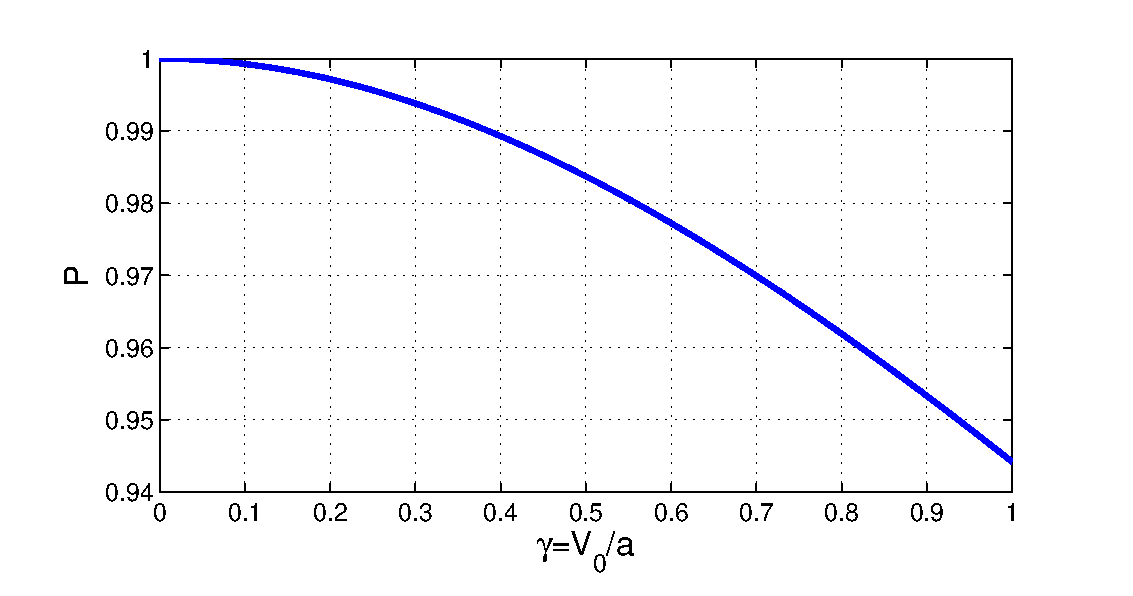
\includegraphics[scale=0.6]{P5_P.eps}
\caption {\small Exact probablity of  emaining in the ground state}
\label{P5-P}
\end{figure}

If we take a look at \eqref{P5-look} we can clearly see that both Hamiltonian are the same and we should just swap $\ket{1}$ & $\ket{2}$ that is those states should be mutually exchanged in our formulation If we reprsents the ground state of the new Hamiltonian as $\ket{\Omega_1}$ then from \eqref{P5-ground} we have:
\begin{equation}
c\ket{\Omega_1}=\left(1-\frac{2\gamma}{9}\right)\ket{2}+\left(1+\frac{\gamma}{9}\right)\ket{1}+\left(1+\frac{\gamma}{9}\right)\ket{3}
\end{equation} 
The probability for the electron to remain in the ground state is:
\begin{equation}
P=\abs{\bracket{\Omega_1}{\Phi_1}}^2\approx\left[\frac{2\left(1-\frac{2\gamma}{9}\right)\left(1+\frac{\gamma}{9}\right)+\left(1+\frac{\gamma}{9}\right)^2}{\left(1-\frac{2\gamma}{9}\right)^2+\left(1+\frac{\gamma}{9}\right)^2+\left(1+\frac{\gamma}{9}\right)^2}
\right]^2
\end{equation}


\end{homeworkSection}

\end{homeworkProblem}


\setcounter{equation}{0}

\newpage

\section{Appendix}
\begin{verbatim}

clc
clear all
close all
 
N=8;          %Number of QW
level=8;      % number of desired mode
%-----------------------------------------------------
Lw=6.25;  
Lb=3.75;
V0=0.9;
%---constants-----------------------------------------------------------
c=300;                       %light speed
h=0.65;                      % reduced plank constant
Meff=0.07*(0.511* 10^6)/c^2; % electron effective mass

%-----Determination of the Energybands (coarse root searching)------------
DE=V0/10^4;
E=[DE:DE:V0-DE];
kw=sqrt(2*Meff*E/h^2);
kb=sqrt(2*Meff*(V0-E)/h^2);
M11=exp(kb*Lb).*(cos(kw*Lw)-0.5*(kw./kb-kb./kw).*sin(kw*Lw));
M22=exp(-kb*Lb).*(cos(kw*Lw)+0.5*(kw./kb-kb./kw).*sin(kw*Lw));
U=abs(0.5*(M11+M22))>1;
n=length(E);
Eg=[];   % Eg is the vector of the edges of the allowable enrgy bands 
swich=1;
for j=2:n
    if(U(j)==0 && swich==1)
       Eg=[Eg E(j)];
       swich=0;
    end
    if(U(j)==1 && swich==0)
       Eg=[Eg E(j)];
       swich=1;
    end
    
    
end
%----------------------------------------------------------------------
Neb=length(Eg)/2;
Ox=[];
Oy=[];
for u=1:Neb
   Ox=[Ox 0 1 1 0];
   Oy=[Oy Eg(2*u-1) Eg(2*u-1) Eg(2*u) Eg(2*u)];
end
figure
fill(Ox,Oy,'r')
Xlim([0 1]);
Ylim([0 V0]);
Ylabel('E(ev)','fontsize',15) % plots energy bands
%---------Determination of the Energy Eigenvalues-------------------------
dE=DE/10^2;
Z=[];
for n=1:Neb
    El=Eg(2*n-1)-DE;
    Eh=Eg(2*n)+DE;
    n
    R=[];
    c=0;
    EE=[El:dE:Eh];
    for E0=El:dE:Eh
    c=c+1;
k1=sqrt(2*Meff*E0/h^2);
k2=sqrt(2*Meff*(V0-E0)/h^2);
M11=exp(k2*Lb).*(cos(k1*Lw)-0.5*(k1./k2-k2./k1).*sin(k1*Lw));
M22=exp(-k2*Lb).*(cos(k1*Lw)+0.5*(k1./k2-k2./k1).*sin(k1*Lw));
M12=-0.5*exp(k2*Lb).*(k1./k2+k2./k1).*sin(k1*Lw);
M21=0.5*exp(-k2*Lb).*(k1./k2+k2./k1).*sin(k1*Lw);
M=[M11 M12;M21 M22];
Mt=M^N;
R=[R Mt(1,1)];

%-------------------

if(R(end)==0)
    Z=[Z E0];
elseif(c==1)
elseif(R(end)*R(end-1)<0)
    Z=[Z E0-dE/2];
end

%-------------------
    end
figure
plot(EE,R,'linewidth',2.5);
Ylim([-0.5 0.5]);
Xlim([El Eh]);
Xlabel('E(ev)','fontsize',15)
Ylabel('M_{11}','fontsize',15)
end

%---------------- Part C- Wavefunction Determination ------------------
Ed=Z(level);
U2=0;
for E0=Ed-dE:dE/100:Ed+dE 
k1=sqrt(2*Meff*E0/h^2);
k2=sqrt(2*Meff*(V0-E0)/h^2);
M11=exp(k2*Lb).*(cos(k1*Lw)-0.5*(k1./k2-k2./k1).*sin(k1*Lw));
M22=exp(-k2*Lb).*(cos(k1*Lw)+0.5*(k1./k2-k2./k1).*sin(k1*Lw));
M12=-0.5*exp(k2*Lb).*(k1./k2+k2./k1).*sin(k1*Lw);
M21=0.5*exp(-k2*Lb).*(k1./k2+k2./k1).*sin(k1*Lw);
M=[M11 M12;M21 M22];
Mt=M^N;

%-------------------

U1=Mt(1,1);
if(U1==0)
    Ed=E0;
    break
elseif(U1*U2<0)
  Ed=E0-dE/2;
   break
end

U2=U1;
end

%-------------------------------------------

%-----------------Mb---------
Mb=zeros(2);
kw=sqrt(2*Meff*Ed/h^2);
q=sqrt(2*Meff*(V0-Ed)/h^2);
Mb(1,1)=exp(q*Lb);
Mb(2,2)=exp(-q*Lb);
%---------------Mwb-----------
Mwb=zeros(2,2);
Mwb(1,1)=1+1i*q/kw;
Mwb(2,2)=Mwb(1,1);
Mwb(1,2)=1-1i*q/kw;
Mwb(2,1)=Mwb(1,2);
Mwb=0.5*Mwb;
%-------------Mw--------------
Mw=zeros(2);
Mw(1,1)=exp(-1i*kw*Lw);
Mw(2,2)=exp(+1i*kw*Lw);
%------------Mbw-------------
Mbw=zeros(2);
Mbw(1,1)=1-1i*kw/q;
Mbw(1,2)=1+1i*kw/q;
Mbw(2,1)=Mbw(1,2);
Mbw(2,2)=Mbw(1,1);
Mbw=0.5*Mbw;
%----------------------------
V1=[1;0];
delta=0.001;
zb=[delta:delta:Lb];
zw=[delta:delta:Lw];
Fb=[exp(-q*zb);exp(+q*zb)];
Fw=[exp(1i*kw*zw);exp(-1i*kw*zw)];
%-----------------------------
z=[];
Y=[];
for(n=1:N)
    if(n~=1)
V1=Mb*Mbw*V2;
    end
z=[zb z];
Y=[V1.'*Fb Y];
z=[zw z+Lw];
V2=Mw*Mwb*V1;
Y=[V2.'*Fw Y];
z=z+Lb;
end
V1=Mb*Mbw*V2;
z=[zb z];
Y=[V1.'*Fb Y];
L=max(z);
x=z-L/2;
figure
Nor=sqrt(trapz(x,abs(Y.^2)));
Max=max(abs(Y)/Nor);

y1=0;
y2=1.2*Max;
Oy=[];
Ox=[];
x1=x(1);
for(m=1:N+1)
    Ox=[Ox x1 x1 x1+Lb x1+Lb];
    Oy=[Oy y1 y2 y2 y1];
    x1=x1+Lb+Lw;
end
fill(Ox,Oy,'g')
Xlim([x(1) x(end)]);
Ylim([0 1.2*Max]);
hold on
plot(x,abs(Y)/Nor,'linewidth',2.5)
Xlabel('x(nm)','fontsize',15)
Ylabel('|\Psi|','fontsize',15)


\end{verbatim}



\end{document}
